%!TEX root = ../slides.tex

\section{Глиальные опухоли}

\begin{frame}
  \frametitle{Глиальные опухоли}
  %\framesubtitle{Subtitles are optional.}
  % - A title should summarize the slide in an understandable fashion
  %   for anyone how does not follow everything on the slide itself.

  \begin{itemize}
  \item \textbf{Нейроглия, или просто глия}  — совокупность вспомогательных клеток нервной ткани. 
  Составляет около 40\% объёма ЦНС. 
  \item \textbf{Астроцит}  — тип нейроглиальной 
  клетки звёздчатой формы с многочисленными отростками. Совокупность астроцитов называется астроглией.
  \item \textbf{Эпендимальные клетки} - напоминают однослойный эпителий, лежат на базальной мембране и 
  имеют кубическую или призматическую форму.
  \item\textbf{Олигодендроциты, или олигодендроглия} — вид нейроглии. Главная функция — 
  предоставлять помощь и изоляцию аксонам нейронов, находящихся в центральной нервной системе позвоночных животных.
  
  
  % 
 \end{itemize}

\end{frame}
\begin{frame}
  \begin{figure}
    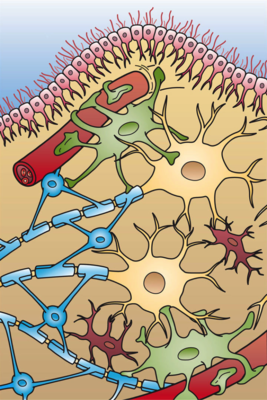
\includegraphics{glia_types.png}
    \caption{Иллюстрация четырёх типов глиальных клеток, находящихся в 
    ЦНС: эпендимный слой (светло-розовый), астроциты (зелёный), клетки микроглии (тёмно-коричневый), олигодендроциты (голубой).}
  \end{figure}
\end{frame}

\begin{frame}
  \frametitle{Глиальные опухоли}

  \begin{itemize}
  \item \textbf{Глиальная опухоль} является патологическим новообразованием, расположенным внутри мозга. 
    Она развивается из глии – вспомогательных клеток нервной ткани.
    
  \item \textbf{Астроцитома} — глиальная опухоль головного мозга, возникающая из астроцитов. 

  \item \textbf{Мультиформная глиобластома} — наиболее частая и наиболее агрессивная форма опухоли мозга,
  которая составляет до 52 \% первичных опухолей мозга и до 20 \% всех внутричерепных опухолей. 

\end{itemize}
\end{frame}

\begin{frame}
  

    \begin{figure}
      \includegraphics[scale=0.06]{Astrocytoma.jpg}
      \caption{Два ПЭТ изображения: верхнее показывает нормальный мозг, а нижнее — с астроцитомой.}
    \end{figure}
  \end{frame}


\begin{frame}
  \frametitle{Глиальные опухоли}  
\begin{itemize}
  

    \item эпендимома — 5-8\% всех опухолей головного мозга (чаще локализуются в желудочковой системе головного мозга)
  \item астроцитома — 50 \% (располагаются обычно в белом веществе головного мозга).
  \item олигодендроглиома — 8-10\%. К ним относятся олигодендроглиома и анапластическая олигодендроглиома
  \item смешанные глиомы (олигоастроцитома, анапластическая олигоастроцитома)
 
   

  \end{itemize}
\end{frame}
\begin{frame}

  \frametitle{Классификация глиальных опухолей}  
  
    \begin{itemize}
      \item I степень злокачественности - доброкачественная опухоль
      \item II степень злокачественности - один признак злокачественности, как правило клеточная атипия
      \item III степень злокачественности - два признака из трех, исключая некрозы
      \item IV степень злокачественности - три или четыре признака, но обязательно наличие некроза
    \end{itemize}
  
  \end{frame}



\begin{frame}
  \frametitle{Симптомы и прогноз}
  \begin{itemize}
    \item Симптомы глиомы являются переменными и зависят от расположения и размера опухоли. 
   

  \item Прогноз относительно выживаемости для данного типа опухолей ЦНС является неблагоприятным. 
  
  \end{itemize}
\end{frame}


\subsection{Методы обследования глиальных опухолей}

\begin{frame}
  \begin{itemize}
    \frametitle{Методы обследования глиальных опухолей}
    \item Компьютерная томография с контрастным усилением (КТ)
    \item Магнитно-резонансная томография  с контрастным усилением (МРТ)
    \item ПЭТ 
    \item Сцинтиграфия
    \item Неврологическое исследование, которое обязательно включает в себя офтальмологическую проверку остроты зрения, глазного дна и полей зрения
    \item Ангиография
  \end{itemize}
\end{frame}